
\documentclass[a4paper,11pt]{article}

\usepackage{amsmath,amssymb,amsfonts,amsthm}    % Typical maths resource packages
\usepackage{graphicx}                           % Packages to allow inclusion of graphics
\usepackage{hyperref}                           % For creating hyperlinks in cross references
\usepackage[authoryear]{natbib}                 % literature reference style
\usepackage[bf, margin=1cm]{caption}
\usepackage[english]{babel}
\usepackage{xcolor} % options: [usenames,dvipsnames]
\usepackage{subfig}
\usepackage{inputenc}
\usepackage[font=small]{caption} 
%\usepackage[showframe]{geometry}

% -------------------------------
% --- for proper tables ---
% -------------------------------

\usepackage{booktabs,
	tabularx,
	ragged2e,
	dcolumn} 

\usepackage{booktabs,tabularx,ragged2e,dcolumn,caption} 
\newcolumntype{C}{>{\Centering\arraybackslash \hspace{0pt}}X}
\newcolumntype{d}[1]{D{.}{,}{#1}}
% handy shortcut macros
\newcommand\mc[1]{\multicolumn{1}{c}{#1}}
\newcommand\MC[1]{\multicolumn{1}{C}{#1}}

% -------------------------------
% --- some layout definitions ---
% -------------------------------

% define topline
%\usepackage[automark]{scrpage2}
%\pagestyle{scrheadings}
%\automark{section}
%\clearscrheadings
%\ohead{\headmark}

% define citation style
\bibliographystyle{ecta}

% define page size, margin size
\setlength{\headheight}{1.1\baselineskip}
%\setlength{\parindent}{0em} 
\voffset=-2cm
\hoffset=-3cm
\textheight24cm
\textwidth15.5cm
\topmargin1cm
\oddsidemargin3cm
\evensidemargin3cm

% comments
\newcommand{\kom}[1]{{\textcolor{red}{#1}}}
\newcommand{\qom}[1]{{\textcolor{green}{#1}}}

% define line line spacing = 1.5
\renewcommand{\baselinestretch}{1.5}

% define second level for `itemizing'
\renewcommand{\labelitemii}{-}

\newtheorem*{lemma*}{Lemma}
\newtheorem*{defin*}{Definition}


% --------------------------------------
% --------------------------------------
% --------------------------------------
% --- the structure the tex document ---
% ---  (this our recommendation) -------
% frontmatter:
%   - titlepage (mandatory),
%   - acknowledgement,
%   - abstract,
%   - table of contents (mandatory),
%   - list of abbreviations (not mandatory),
%   - list of figures (not mandatory),
%   - list of tables  (not mandatory) .
%
% body of the thesis (the structure of the thesis body is not mandatory, but the list of literature is mandatory):
%   - introduction,
%   - methods,
%   - data,
%   - results,
%   - conclusion,
%   - literature (mandatory),
%   - appendix (figures, tables).
%
% last page:
%   - declaration of authorship (mandatory).
% --------------------------------------
% --------------------------------------
% --------------------------------------

\begin{document}

% -------------------------------
% --- frontmatter: Title page ---
% -------------------------------

\thispagestyle{empty}
%\begin{center}
%	
%	\begin{figure}[htb!]
%		\centering
%		\includegraphics[width=0.8\textwidth]{logo}
%	\end{figure}
%	
%
%    {\LARGE{\bf Mitigating Covariate Shift for Low Dimensional Machine Learning Problems via Lattice Based Models}} \vspace{0.5cm}
%	\vspace{0.5cm}
%	
%	{\LARGE Bachelor's Thesis}
%	
%	{\normalsize in partial fulfillment for acquiring \\
%		the degree of \medskip
%		{\bf Bachelor of Science} (B.Sc.)\medskip
%		in Economics \medskip
%	Chair of Information Systems \\
%    School of Business and Economics \\
%    Humboldt-Universit\"at zu Berlin} \vspace{1cm}
%
%
%    {\normalsize by \\\vspace{0.5cm}
%    {\bf Jonathan Schmitz} \\
%    591778 \vspace{1cm}}
%
%
%    
%    
%    Berlin, \kom{September 30, 2007}
%
%\end{center}

\begin{center}
	
		\begin{figure}[htb!]
			\centering
			
\includegraphics[width=0.3\textwidth]{img/pepe}
		\end{figure}
	\vspace*{0.5cm}
	
	{\Large{\bf Mitigating Covariate Shift for Low Dimensional Machine Learning Problems via Lattice Based Models}} \vspace{0.5cm}
	
	
	{\normalsize Bachelor's Thesis submitted\\\vspace{0.5cm}
		to}\\\vspace{0.5cm}
	{\normalsize{\bf Prof. Dr. X Man}} \\\vspace{0.5cm}
	
	{\normalsize Infinite-Jest-Universität zu Berlin \\
		School of Joy and Fun \\
		Chair of Entertainment Systems}  \vspace{1cm}
	
	
	{\normalsize by \\\vspace{0.5cm}
		{\bf jvosten} \\
		654321 \vspace{1cm}}
	
	
	{\normalsize in partial fulfillment for acquiring \\
		the degree of \\
		{\bf Bachelor of Science} (B.Sc.) \\
		in Economics \vspace*{0.75cm}
		
		Berlin, February 29$th$, 2021}
	
\end{center}

% ------------------------------------
% --- frontmatter: Acknowledgement ---
% ------------------------------------
\newpage
%\input{prependix/glied}

%
%% -----------------------------
%% --- frontmatter: Contents ---
%% -----------------------------
\newpage
\pagestyle{plain}
\pagenumbering{roman}   % define page number in roman style
\setcounter{page}{1}    % start page numbering
\tableofcontents
\clearpage
%

%
% -------------------------------
% --- main body of the thesis ---
% -------------------------------
\newpage
\pagestyle{plain}
\setcounter{page}{1}    % start page numbering anew
\pagenumbering{arabic}  % page numbers in arabic style

%\fcolorbox{red}{yellow}{\begin{minipage}{\textwidth}
%		
%\end{minipage}}

\section{Introduction}\label{Sec:intro}

In recent years \textit{data} has become an important topic for the broader public, exceeding its natural habitat of science and computer programming. Some proclaimed it to be the oil of the $21{th}$ century. A major reason for the rush lies in the availability of data and the development of new technologies and methods, which enable us to design algorithms that learn from data. This emerging scientific field is known as Machine Learning (ML), some even see the advent of a new scientific age:
\begin{quote}
	\small
	The new availability of huge amounts of data, along with the statistical tools to crunch these numbers, offers a whole new way of understanding the world. Correlation supersedes causation, and science can advance even without coherent models, unified theories, or really any mechanistic explanation at all.\footnote{\url{https://www.wired.com/2008/06/pb-theory/}}
\end{quote}
To temper the above quoted author's excitement, we could simply ask about the Problem of Induction; the question of whether it is possible to infer a generally valid law based on single observations. Presuming we go bird watching and observe a 100 swans, all of them with white plumage, we could then draw the following two inductive conclusions:
\begin{quote}
	\begin{itemize}
		\small
		\item[(C1)] All swans observed so far were white. Therefore all swans are white.\\ $F(a_1),\dots, F(a_n) \Rightarrow \forall x: F(x)$. 
		\item[(C2)] All swans observed so far were white. Therefore the next observed swan will be white. $F(a_1),\dots,F(a_n) \Rightarrow F(a_{n+1})$.
	\end{itemize}
\end{quote} 
This poses two questions regarding justification: how do we justitfy generalizing about some object $x$'s features $F$ based on $n$ observations of a particular instance $F(a_1),\dots,F(a_n) $; and how do we justify the assumption, that future observations $a_{n+1}$ are going to fall under $F$, as the past ones. The \textit{Problem of Induction} forms one of the fundamental problems in the domain of Epistemology and Theory of Machine Learning \cite{sterkenburg2020no}. In bringing this up, we remark that (statistical) learning from data faces the same problems as any field utilizing inductive inferrence. Regarding ML we could then alter $C1$ and $C2$ in the following way
\begin{quote}
	\begin{itemize}
		\small
		\item[(C3)] All observations $x_i$ for feature $x$ fall within the range of $[a,b]$. Therefore the model learns $y \in [a,b]$. 
		\item[(C4)] All observations $x_i$ for feature $x$ fall within the range of $[a,b]$. Therefore the model predicts $y \in [a,b]$ for $x_{n+1}$.
	\end{itemize}
\end{quote} 
One could insist that the reasoning of $C3$ and $C4$ does not seem problematic and refers us to all those well-functioning ML models and applications. But, especially when it comes to real world ML applications, the following problem is very common: the data $x_{ts} \in [c,d]$, on which the model $f(x)$ will be tested on in the end by the user, is not strictly (or not at all) represented by the data $x_{tr} \in [a,b]$ that was used  for training the underlying model. This kind of violation of $C3$ and $C4$ is called Dataset Shift \citep{moreno2012unifying}. More technically speaking, dataset shift appears when training and test joint distributions are different \citep{quionero2009dataset}. Moreno-Torres et al. identify three main types of dataset shift, covering ($i$.) a shift in the independent variables (\textit{Covariate shift}), ($ii$.) in the target variable (\textit{Prior probability shift}) or ($iii$.) in the relationship between the two (\textit{Concept shift}) .

In this paper we will focus on the first type, covariate shift. In this case the values of the covariates $X$ causally determine the class label $Y$. A shift then occurs, if the distribution of one or more of the covariates $X_{ts}$ in the test data significantly changes compared to $X_{tr}$ in the training data. Our goal then is to employ a monotonic lattice based model to mitigate the effect of covariate shift. This kind of model learns flexible monotonic functions by using calibrated interpolated look-up tables, the lattice \citep{gupta2016monotonic}. We can think of it as looking up a value $x$ for $\mathrm{sin}(x)$ in a textbook. The monotonicity constraint for individual features allows us to model prior knowledge. For instance, assume we want to estimate the risk of lung cancer for a patient. In the patients record we might find a covariate `cigarettes smoked per day'. We expect the risk of lung cancer never to decrease as the amount of cigarettes smoked per day increases. This prior domain knowledge could nout be reflected in a model that learns from a small and noisy data set (see also the example of Fig. \ref{Fig:gup2} and \ref{Fig:gup1}).

There is one major restriction to the lattice approach, though. It is only suitable for low dimensional ML problems, because the weights of the function are computed in $\mathcal{O}(2^D)$ operations. For the experiment in this paper we will use data from the domain of credit scoring, as the information on potential customers, characterized by the covariates, determines the credit score $Y$. Credit scroing is very suitable for our endeavour, as it can be considered a low dimension setting \citep[Tab.~1]{lessmann2015benchmarking} and covariate shift can be a problematic issue (see \ref{Sec:covshift}). The goal of the experiment is to show that a TensorFlow Lattice (TFL) calibrated linear model (GAM) does not perform worse than a comparison classifier, in this case a Random Forrest model.

The paper is organized as follows. We begin with an overview of relatedwork in covariate shift adaption. Then we outline the theoretical conception of covariate shift, lattice regression and extionsions of the lattice model. Sec. \ref{Sec:Exp} describes the experiment set-up, followed by a presentation of the results. Finally, we draw a conclusion in  Section \ref{Sec:Conc}. 
		
\section{Related Work}\label{Sec:Relwork}

Since mitigation of covariate shift is the main topic of this paper, the literature review is going to be focused on this aspect. For a review of similar learning methods as the montonic calibrated lattice applied here, see \citep{gupta2016monotonic}. For a review of classifier selection for credit scoring, see \cite{baesens2003benchmarking} respectively \citep{lessmann2015benchmarking}.

We furthermore restrict our literature review to methods dealing with what \citep{storkey2009training} calls `Simple covariate shift' (p. 7) in the pardigm of unsupervised learning; that is if the complete data set shift is characterized by what we will define as covariate shift in Sec. \ref{Sec:covshift}: $P_{tr}(x) \neq P_{tst}(x)$, everything else stays the same. Exceeding this rather simple case of data set shift there exists a broad literature on domain and method specific ways to mitigate cases in which covariate shift is only one aspect of bias; see for instance \citep{kato2020off} or \citep{johansson2018learning}.

As we will see in Sec. \ref{Sec:covshift} there is no general definition for covariate shift, neither is there even a common naming convention for the general problem of data set shift \citep{moreno2012unifying}. This makes it complicated to compile a review of the literature on the topic, as some work could have been overseen simply because of the aforementioned. Apart from this we can identify two superordinated approaches for covariate shift correction: ($i$.) importance weighting and ($ii$.) error bounds for domain adaption (statistical learning bounds).


\subsection*{Importance Weighting}

Given we know the probabilites of finding $x$ in the train and test set, $P_{tr}(x)$ and $P_{tst}(x)$, \citep{shimodaira2000improving} showed that under covariate shift the log-likelihood estimation becomes asymptotically optimal, if each instance is reweighted with 
\begin{align*}
	w(x) = \frac{P_{tst}(x)}{P_{tr}(x)}. 
\end{align*}

An individual training point $x_i$ receives a higher weight, if its probability of appearing in the test set is high. Multiplying the resulting weights with the initial input is supposed to result in a more accurate prediction.  \citep{nair2019covariate} give an overview on the most important methods for estimating $w(x)$ following the above sketched \textit{Importance Weighting}:

\begin{description}
	\item[Discriminative Learning] \citep{bickel2009discriminative} propose to use a probabilistic classifier for estimating $w(x)$. The probabilites are estimated by a discriminative algorithm; they can furthermore be utilized as a measure to decide upon the existence of covariate shift for the data set of concern. More efficient versions of this method have been introduced by \citep{sugiyama2010superfast} (least-squares probabilistic classifier) and \citep{yamada2011improving} (importance weighted LSPC).
	
	\item[Kernel Mean Matching] Here training and test data are mapped to reproducing kernel Hilbert spaces (RKHS) and distances between mappings are measured. The algorithm then reweights the training data in a way that their RKHS mapping corresponds to that of the test data \citep{gretton2009covariate}, \citep{huang2006correcting}. This approach has the advtange that no estimation of the densities is required. It got extended by \citep{kanamori2009condition} and \citep{miao2015ensemble}. 
	
	\item[KLIEP] (\textit{Kullback Leibler Importance Estimation Procedure}) Model Selection for the above KMM method may be biased. \citep{sugiyama2008direct} therefore propose a method that directly estimates $w(x)$ without density estimation and that contains a proper model selection, by minimizing the Kullback-Leibler divergence from $P_{tst}(x)$ to its estimate $\hat{P}_{tst}(x) = \hat{w}(x)P_{tr}(x)$.
	
	\item[(u)LSIF] \textit{(Unconstrained) Least Squares Importance Fitting (uLSIF)} Similar method as KLIEP that uses squared loss to model the importance estimation \citep{kanamori2009least}. It is supposed to be more efficient then KLIEP. uLSIF is a numerically stable version of LSIF.
\end{description}

In addition, there are further approaches to the problem, as \textit{Asymptotic Bayesian Generalization Error} \citep{yamazaki2007asymptotic}, \textit{Importance Weighted Cross Validation} \citep{sugiyama2007covariate} or \textit{Adversarial Search} \citep{globerson2009adversarial}.

\subsection*{Statistical Learning}

\citep{bendavid2009training} provides a setting of domain adaption for which he derrives error bounds. These bounds forego assumptions on the similarity between the domain of train and test data. Ben-David proposes two different algorithms, which he calls `adaptive inductive transfer learning algorithms', see \citep{ben2003exploiting} and \citep{ben2007analysis}.
\bigskip

In addition, an exhaustive overview on covariate shift adaption can be found in \citep{sugiyama2012machine}.

\section{Theoretical Foundations}\label{Sec:Method}

In this section we provide a brief introduction into covariate shift and illustrate, how it can be related to credit scoring. In the subsections below, we will then explore the lattice regression framework and its monotonicity and calibration extensions.

\subsection{Covariate Shift}\label{Sec:covshift}

In supervised machine learning, it is often assumed that the test and training data follow the same distributions, or that it does not matter if their domains do not match. In real-world applications this mismatch can lead to models performing well in a certain context, but failing in other contexts, where, compared to the training context, the data shifted. Data set shift therefore describes the effects of the violation of the above mentioned assumption. In the literature there are several approaches to systemize data set shift: \citep{storkey2009training} describes causes of data set shift, \citep{moreno2012unifying} systemize four different effect types of shift (the three types stated in Sec. \ref{Sec:intro} plus `other types') and \citep{kull2014patterns} refine the aforementioned approaches by extending the categorization and by supplementing it with a formal notation using graphical models. For our purpose it will be sufficient to refer to the simple distinction of shifts as described by Moreno-Torres et al., as the specifications of Kull and Flach concern relatively particular cases. 

\citep{moreno2012unifying} model dataset shift as a change in the joint probability distribution $P(y,x)$ of the covariates $X$ and the labels $Y$: 
\begin{quote}
	{\it \textbf{Dataset shift} appears when training and test joint distributions are different. That is, when $P_{tr}(y,x) \neq P_{tst}(y,x)$.}
\end{quote}

The authors give a further specification of the joint distribution $P(y,x)$ to take into consideration the causal relationship between covariates and class labels. The kind of shift that is possible depends on the structure of the problem, leading to the distinction of two cases: for $X \rightarrow Y$ problems values of covariates causally determine the class label; for $Y \rightarrow X$ problems class labels determine the values of covariates. For the former the joint probability distribution $P_{tr}(y,x) = P_{tst}(y,x)$ can then be written as $P(y|x)P(x)$, for the later as $P(x|y)P(x)$. 

From the above Moreno-Torres et al. obtain a formal definition of covariate shift:
\begin{quote}{ \it
	\textbf{Covariate shift} appears only in $X \rightarrow Y$ problems, and is defined as the case where $P_{tr}(y|x) = P_{tst}(y|x)$  and $P_{tr}(x) \neq P_{tst}(x)$.}
\end{quote}
Here only the distributions of $x$ for test and train sets change, the functional relationship of the model stays the same. For a mathematical more rigorous description of the entire problem setting see \citep{sugiyama2012machine}. The definitions of the other types of shift are summarized in Tab. \ref{Tab:dataset_shift}. 

\begin{table}[ht]
	\begin{center}
		{\footnotesize
			\begin{tabular}{lcccc}
%				\toprule
%				& $X \rightarrow Y$ Problem & & $Y \rightarrow X$ Problem & \\
%				\hline
%				& $P_{tr}(y|x) = P_{tst}(y|x)$ & $P_{tr}(x) = P_{tst}(x)$    & $P_{tr}(x|y) = P_{tst}(x|y)$     & $P_{tr}(y) = P_{tst}(y)$  \\
%				\hline
				\toprule
				\multicolumn{1}{c}{ } & \multicolumn{2}{c}{$X \rightarrow Y$ Problem} & \multicolumn{2}{c}{$Y \rightarrow X$ Problem } \\
				\cmidrule(l{3pt}r{3pt}){2-3} \cmidrule(l{3pt}r{3pt}){4-5} 
				& $P_{tr}(y|x) = P_{tst}(y|x)$ & $P_{tr}(x) = P_{tst}(x)$    & $P_{tr}(x|y) = P_{tst}(x|y)$     & $P_{tr}(y) = P_{tst}(y)$  \\
				\midrule
				Covariate Shift   & True & False & -- & --   \\
				Prior Probability Shift  & -- & -- & True & False \\
				Concept Shift & False & True & False & True\\
				Other types & False & False & False &False \\
				\bottomrule
		\end{tabular}}
	\end{center}
	\caption{The four types of dataset shift displayed in form of a logical truth table for both kinds of problem. Each depicted case leads to $P_{tr}(y,x) \neq P_{tst}(y,x)$.} 
	\label{Tab:dataset_shift}
\end{table}



To illustrate the relationship between covariate shift and credit scoring we draw on an example from \citep[Sec.~8.2]{wang2020deontological}. Here, a credit scoring model is employed based on the Taiwanese UCI Credit Card data set, which we also will use for our experiment in Sec. \ref{Sec:Exp}. The authors remark a potenital bias for the variable `Repayment status (April)', as the data appears to be very noisy for cases with $overdue > 3$ (see Appendix Fig. \ref{Fig:gup3}). In a simplified two-feature test case (with covariates `Marital status' and `Repayment status (April)') their model then yields the output visualized in Fig. \ref{Fig:gup2}:

\begin{figure}[htb!]
	\centering
	\begin{minipage}{0.45\textwidth}
		\centering
		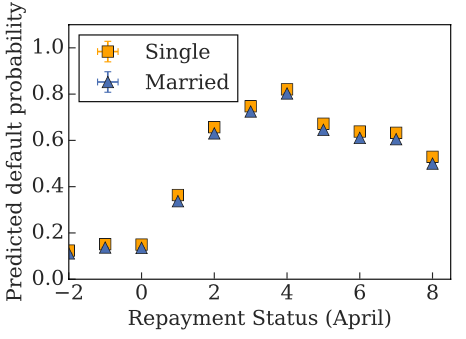
\includegraphics[width=1\textwidth]{img/gup2} % first figure itself
		\caption{Baseline model}
		\label{Fig:gup2}
	\end{minipage}\hfill
	\begin{minipage}{0.45\textwidth}
		\centering
		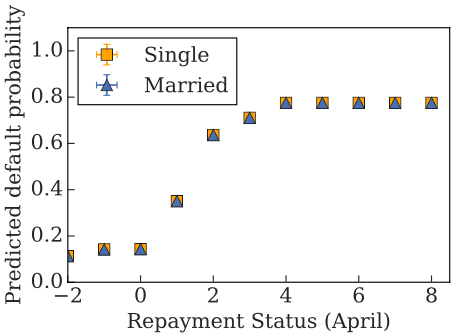
\includegraphics[width=1\textwidth]{img/gup1} % second figure itself
		\caption{Lattice model}
		\label{Fig:gup1}
	\end{minipage}
\end{figure}

Fig. \ref{Fig:gup2} shows that customers who are 5 or 6 month overdue, are assigned a lower score than those, who are only 2 months overdue. This means, borrowers are penalized by the score for paying back in time. The underlying bias most likely results from the training data only containing 122 cases of $overdue > 3$, leaving those cases underrepresented in a training set of 30.000 observations. We can then model this example as a case of covariate shift.  

Assume we now want to apply the classifier in a new context. In our new test set there is a significantly higher amount of observations with $overdue > 3$ for `April repayment', let it be 5\% instead of 0.4\%. We then have $P_{tr}(\mathrm{April\ repayment}) \neq P_{tst}(\mathrm{April\ repayment})$, potentially penalizing those customers who are only slightly overdue. All other variables fixed, those customers obtain a worse credit score then heavy overdue customers. The functional relationship $P(y|x)$ remains unchanged, but the input distribution $p(x)$ differs. 

To mitigate the bias of the estimator, Wang and Gupta supplement their lattice model with a \textit{mononicity shape constraint}. In Fig. \ref{Fig:gup1} we see a more consistent behaviour of the estimator, as the shape constraint permits to integrate prior knowledge into the model. For their experiment the authors used a nonlinear generalized additive model, respectively a TFL calibrated linear model. In the following subsections we explore the concept behind the lattice modeling approach.

\subsection{Lattice Regression}

\textit{Lattice regression} is the name for a regression method, in which the estimated function is represented as a rectangular grid of function values spanning the input domain. As in a textbook lookup table for the $z$-values of standard normal distribution, any needed value can then be linearly interpolated from the lattice. In developing supervised machine learning applications we usually start from scratch fitting a function $f(x)$ to the available training data by using some regression algorithm, with the data consisting of randomly sampled pairs $\{(x_i, y_i)\}$. In a second step $f(x)$ can then be evaluated on a lattice to generate a look up table. There is a disadvantage to this two-step procedure, though, as the effect of interpolation from the lattice nodes (on the error of the training samples) is not taken into account, respectively the empirical risk function does not consider the interpolation step. To solve this issue, \citep[pp.~1]{garcia2009lattice} 
\begin{quote}\small
	propose a solution that we term lattice regression, that jointly estimates lattice outputs by minimizing the regularized interpolation error on the training data. [...] The key to this estimation is that the linear interpolation operation can be directly inverted to solve for the node outputs that minimize the squared error of the training data.
\end{quote}
The major constraint of this approach is the exponential scaling of the interpolation operation with $\mathcal{O}(2^D)$, as each evaluation of $f(x)$ calls for the interpolation of the $2^d$ lattice nodes. Therefore lattice regression rather suits low-dimensional problems. 

 In the following subsections we will provide an overview on lattice regression. At first we take a look at the regression objective; then we will describe the interpolation function for the function output and last we present different regulizers for the estimation function.

\subsubsection{Regression Objective}

In regression we commonly try to estimate a function $\hat{f}:D \rightarrow \mathbb{R}$ within some class of functions $\mathcal{F}$ to minimize the empirical risk $\sum \ell(y, \hat{f}(x))$ for some loss funtion $\ell(\cdot)$. In lattice regression the class of admissible functions $\mathcal{F}$ is then restricted to the following: given the bounded input space $D \subset \mathbb{R}^d$ (with $d = 1, \dots, D$ being the amount of covariates) from which we draw the training data with inputs $\{x_i \in D\}_{i=1:n}$ and outputs $\{y_i \in \mathbb{R}\}_{i=1:n}$. We then assume a lattice spanning the domain $D$, consisting of $M = \prod_{d} M_d = M_1 \times M_2 \times \dots M_D$ vertices, whereby $M_d \in \mathbb{N}$ is to be considered a hyperparameter which determines the number of vertices in the lattice for the \textit{d}th covariate. Each individual vertex of $M$ then consists in an input-output pair $(v_j \in \mathbb{R}^d, \theta \in \mathbb{R}^M)$, with the inputs $v_j$ forming a lattice that spans the hyper-rectangle $\mathcal{M} \triangleq [0, M_1 - 1] \times [0, M_2 -1] \times \dots [0, M_D -1]$ and the outputs $\theta$ which are the learned lattice values of $f(x)$. For reasons of notational simplicity we follow \citep{gupta2016monotonic} and assume a $2^D$ lattice such that $x \in [0,1]^D$; furthermore we follow \citep{garcia2012optimized} assuming a domain transformation to obtain a lattice with one corner placed at the origin and regularly spaced vertices. Fig. \ref{Fig:int} shows such a $2^D$ lattice with $D=2$. Then the class of admissible functions $\mathcal{F}$ is restricted by those functions `that can be implemented by linearly interpolating a rectangular lattice' \citep[Sec.~2]{garcia2012optimized}.  Finally any function in $\mathcal{F}$ is fully defined by the output set $\{\theta\}$, given lattice inputs $\{v_j\}$ and a linear interpolation method for calculating the interpolation weights $\phi(x)$. 

For linear interpolation of $x_i$ the interpolation weights $\phi(x_i)$ are calculated. The sum of these weight vectors can be written as a uniquely determined matrix $\phi(x) \in [0,1]^{n\times M}$, as they depend on the lattice vertices $\{v_j\}$ and the input data $\{x_i\}$. To be more precise, the set of linear interpolation weights $\phi(x)$ is the solution to the following system of equations:
\begin{equation}
\sum_{k=0}^{2^D} \phi_k(x_i) v_k = x_i\ \mathrm{and}\ \sum_{k=0}^{2^D} \phi_k(x_i) .
\label{Eq:latregsys}
\end{equation}
As we obtain $\theta$ through $\phi(x)$, we can finally compute $\hat{f}(x_i) = \theta^T \phi(x_i)$. The goal of lattice regression is then to minimize the interpolation error on the training data, ergo to minimize the empirical risk function by solving for lattice output $\theta$: 
\begin{align}
\hat{\theta}& = arg\ \underset{\theta \in \mathbb{R}^M}{min} \sum_{i = 1}^{n} \ell(y_i, \hat{f}(x_i)) \nonumber \\
& = arg\ \underset{\theta \in \mathbb{R}^M}{min} \sum_{i = 1}^{n} \ell(y_i, \theta^T \phi(x_i)).
\label{Eq:latregob1}
\end{align}
Assuming squared loss $\ell(y,z)=(y-z)^2$ for the loss funcion $\ell$ in the empirical risk alters Eq. \ref{Eq:latregob1} into the following equation:
\begin{align}
\hat{\theta} = arg\ \underset{\theta \in \mathbb{R}^M}{min} \left\| y - \theta^T \phi(x) \right\|_2^2.
	\label{Eq:latregsql}
\end{align}
Eq. \ref{Eq:latregsql} yields us the objective function of a linear regression model which finds a solution in $(\phi(x)^T\phi(x)^{-1})\phi(x)^T y$. If Eq. \ref{Eq:latregsql} is underdetermined, there is no solution. \citep{garcia2012optimized} remark this to be the case often. There are for instance cases, in which $\phi(x)$ will not be invertible, leaving Eq. \ref{Eq:latregsql} with an infinite set of minimizers. To prevent this problem and further to reduce overfitting to the training data, a graph regulizer $R(\theta)$ is added to the regression objective. Before we examine potential regulizers, we take a closer look at the interpolation function $\phi(x_i)$ in the following subsection, as it will help use to gain a deeper understanding of lattice regression.


\subsubsection{Interpolation}

For interpolation \citep{garcia2009lattice} propose a method called \textit{multilinear interpolation}. Any test point $x \in D$ is contained in one of the cells of the lattice, more precisely, any $x$ is surrounded by $2^D$ vertices from which the lattice output $\theta$ will be then interpolated.
\begin{figure}[htb!]
	\centering
	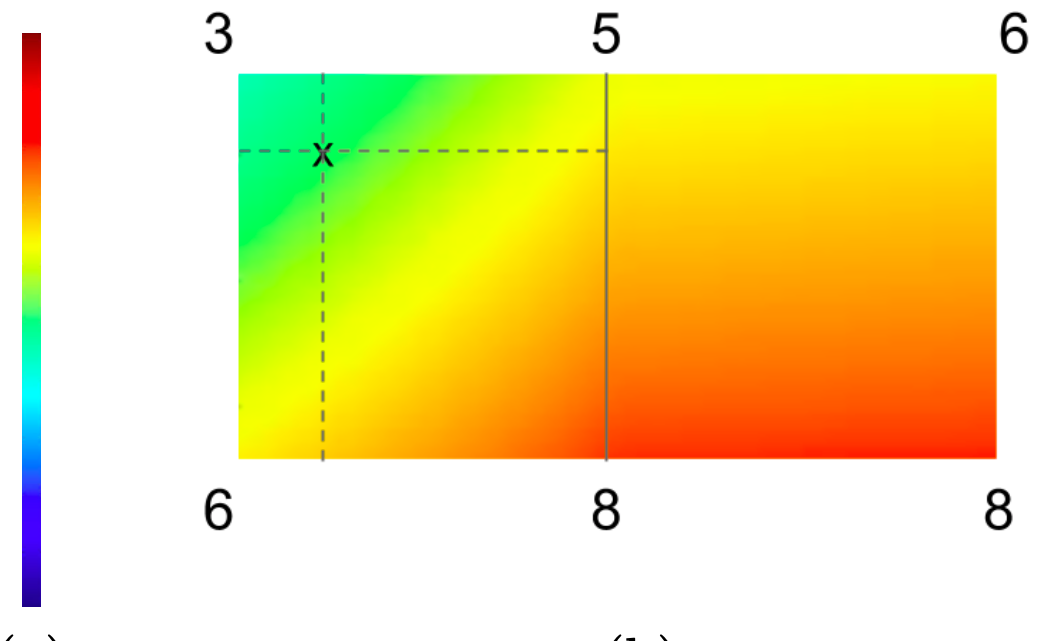
\includegraphics[width=0.5\textwidth]{img/interpol} % first figure itself
	\caption{Example for a $D = 2$ lattice function $f(x)$. Assuming (a) would be scaled with $[0, 1]$, then $f(x)$ would be approx. a value of $0.5$ \citep{gupta2016monotonic}.}
	\label{Fig:int}
\end{figure}
 Fig. \ref{Fig:int} shows the simple case of a $2 \times 2$ lattice; to evaluate the lattice function, $x$ is linearly interpolated from parameter values $\theta = (6, 8, 3, 5)$ at the vertices $v_1, v_2, v_5, v_6$. The interpolation method therefore consists of a linear combination $\phi_k(x) = [\phi_1(x), \dots \phi_{2^D}(x)]^T$ of the surrounding vertice outputs $\theta$. \citep[p.~3]{gupta2016monotonic} give a very concise graphical description of the functioning of the weighting for low dimensional cases as in Fig. \ref{Fig:int}: \begin{quote} \small
	The weights on the parameters [at the vertices] are the areas of the four boxes formed by the dotted lines drawn orthogonally through $x$, with each parameter weighted by the area of the box farthest from it, so that as $x$ moves closer to a parameter the weight on that parameter gets bigger.
\end{quote} 
To interpolate any point $x$ we first need to be able to index its surrounding lattice cell. To obtain the \textit{k}th vertex of the lattice cell, that surrounds $x$, a function $c_k(x): \mathbb{R}^{d} \rightarrow \mathbb{N}$ (for details on its computation see \citep{garcia2012optimized} is defined.  Let then $v_{c_k(x)}\ for\ (k = 1, \dots, 2^D)$ be the \textit{k}th vertex of the lattice cell containing $x$. The associated weights $\phi_k(x)$ for that cell can then be computed as
\begin{equation}
\phi_k(x) = \prod_{d=0}^{D-1} x[d]^{v_k[d]}(1- x[d])^{1-v_k[d]}.
\label{Eq:latregint}
\end{equation}
Note that we assumed a $2^D$ lattice, in this case $v_k \in \{0,1\}^D$ can be seen as the \textit{k}\ th vertex of the unit hypercube (the logic stays the same for multi-cell lattices, the formulas can be looked up in \citep{garcia2012optimized}. The exponent functions as a bitwise selector, multiplying one of the two $x[d]$ terms. We can then form the $M \times 1$ sparse weight vector for each observation $x_i$:
\begin{equation}
	\phi(x_i)[d] = \begin{cases}
	\phi_k(x_i) & \text{if } d = c_k(x_i),\ \text{for } k = 1, \dots, 2^D\\
	 \mspace{18mu} 0 &  \text{otherwise}.
	\end{cases}
\end{equation}
The function value for $x_i$ is then interpolated as $\theta^T \phi(x_i)$; concatenating all these individual vectors yields us a matrix, which can be described as the lattice function $\theta^T \phi(x)$. In addition, we can think of it as a kernel method that maps $x$ to a transformed feature vector $\phi(x)$. Garcia and Gupta chose \textit{d}-linear interpolation as method, because it can be implemented efficiently and it is the maximum entropy solution to Eq. \ref{Eq:latregsys}. \citep{gupta2016monotonic} also accredit the $\theta$ parametrization an improved interpretability effect. In addition they propose two new methods for faster interpolation (with \textit{simplex} interpolation requiring $\mathcal{O}(D log D)$ operations instead of $\mathcal{O}(D2^D)$, as with d-linear interpolation). To complete the lattice regression method we still need to supplement Eq. \ref{Eq:latregob1} with a regulizer term.

\subsubsection{Regulizer}

With the purpose to reduce over-fitting to the training data and to ensure a unique solution to Eq. \ref{Eq:latregob1} \citep{garcia2012optimized} introduce two kinds of graph regulizers $R(\theta)$. On the one hand there is the \textit{graph Laplacian} regulizer: 
\begin{equation}
	R_{laplacian}(\theta) = \sum_{adjacent\ v_r, v_s} 
	(\theta_r - \theta_s)^2 
	= \theta^T\mathbf{K}_L\theta.
	\label{Eq:latreglap}
\end{equation}
Here, the sum of squared differences between the lattice values $\theta$ at adjacent vertices $v_j$ is penalized.  Multiplying Eq. \ref{Eq:latreglap} with a regularization paramater $\lambda > 0$ (smoothness/accuracy trade off) and adding it to the regression objective of Eq. \ref{Eq:latregob1}, this yields a closed form solution $(\phi(x)^T\phi(x)^{-1} + \lambda \mathbf{K}_L)\phi(x)^T y$. %\medskip

\begin{figure}[htb]%
	\centering
	\subfloat[Laplacian]{{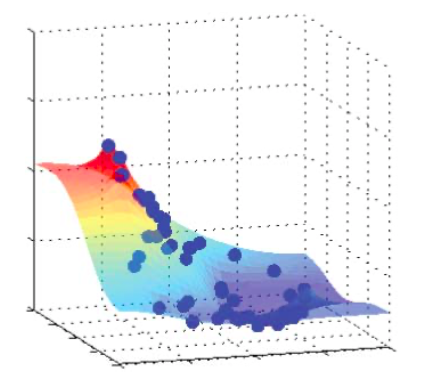
\includegraphics[height=4cm]{img/reg1} }}%
	\hspace{2cm}
	\subfloat[Hessian]{{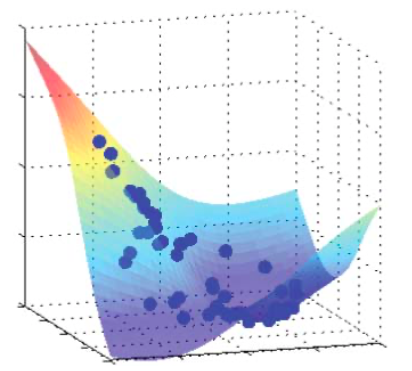
\includegraphics[height=4cm]{img/reg2} }}%
	\caption{Implementation of two regulizers on the same training data (blue dots). \citep{garcia2012optimized}}%
	\label{Fig:reg1}%
\end{figure} 

Garcia and Gupta argue that the Laplacian regulizer is not optimal, as it penalizes the estimation of linear functions. Therefore they propose a regulizer which penalizes the second-order difference in each dimension of the lattice:

\begin{equation}
		R_{hessian}(\theta) = \sum_{d=1}^{D}
		\sum_{\substack{v_r, v_s, v_t\\ adjacent\ in\\ dimension\ d}} 
		((\theta_t - \theta_r) - (\theta_r - \theta_s))^2
		= \theta^T\mathbf{K}_H\theta.
		\label{Eq:latreghes}
\end{equation}

They refer to Eq. \ref{Eq:latreghes} as \textit{graph Hessian} regulizer. In the same way as Laplacian regulizer it yields a closed form solution to \ref{Eq:latregob1}: 
\begin{equation*}
	(\phi(x)^T\phi(x)^{-1} + \lambda \mathbf{\tilde{K}}_H)\phi(x)^T y\quad \mathrm{with}\quad \tilde{K}_H = K_H + 10^{-6}\mathbf{I}. 
\end{equation*}
What is the difference to the Laplacian? Fig. \ref{Fig:reg1} shows how the Hessian regulizer permits linear extrapolations, whereas the Laplician penalizes them. 

Furthermore, \citep{gupta2016monotonic} propose a third type of regulizer; it functions in a similar way as the Hessian regulizer, making the function more linear. For a concise comparison of all three regulizers, see p. 20.\medskip 

With the regulizer at hand, the lattice regression objective has the following form:
\begin{equation}
arg\ \underset{\theta \in \mathbb{R}^{M}}{min} \sum_{i = 1}^{n} \ell(y_i, \theta^T \phi(x_i)) + R(\theta).
\label{Eq:latregob2}
\end{equation}

Regarding the credit score example from Sec. \ref{Sec:intro} the above objective function is just the base framework. To obtain the full functionality of the TFL calibrated model we will use for the experiment in Sec. \ref{Sec:Exp}, Eq. \ref{Eq:latregob2} has to be augmented with \textit{monotonicity constraints} and \textit{feature calibration}. We briefly introduce both additions in the following subsection.

%\begin{equation}
%	R_{torsion}(\theta) = \sum_{d=1}^{D}
%	                            \sum_{\substack{\tilde{d}=1\\
%	                            \tilde{d}\not= d}}^{D}\;
%	                            \sum_{\substack{r,s,t,u\ such\ that\\
%			                    v_r\ and\ v_s adjacent\ in\ dim.\ d,\\ 
%	                            v_t\ and\ v_u adjacent\ in\ dim.\ d,\\
%                                v_r\ and\ v_t adjacent\ in\ dim.\ \tilde{d}}} 
%                                ((\theta_r - \theta_s) - (\theta_t - \theta_u))^2 
%                                = \theta^T\mathbf{K}_T\theta
%\end{equation}



\subsection{Lattice Framework Extensions}

The extension of lattice regression to monotonic functions and jointly learning covariate calibration was proposed by \citep{gupta2016monotonic}. For our case study we will use a TFL linear model which is monotonically constrained and calibrated; therefore we are give a brief overview on both in the next two subsections. 

\subsubsection{Monotonicity}

For the problem setting of lattice regression Gupta et al. give the following definition for monotonicity:
\vspace*{-1cm}
\begin{quote}
	\begin{defin*}
		A function $f(x)$ is monotonically increasing with respect to feature $d$ if $f(x_i) \geq f(x_j)$ for any two feature vectors $x_i,x_j \in \mathbb{R}^D$ where $x_i[d] \geq x_j[d]$ and $x_i[m] = x_j[m]$ for $m \neq d$. 
	\end{defin*}
\end{quote}
Monotonic constraints are applied to machine learning problems to impose prior knowledge and also regularize the estimated functions. Fig. \ref{Fig:mon1} shows an example of an applied constraint. Gupta et al. give an extinsive overview of the related literature concerning the learning of monotonic functions.

For lattice regression, the goal is to ensure that a monotonic function is learned. Therefore some constraints have to be imposed on lattice output parameters $\theta$ during the learning process. For a $2^D$ lattice to be monotonically increasing in the \textit{d}th covariate Gupta et al. give the following lemma for the monotonicity constraints (p. 12):
\vspace*{-1cm}
\begin{quote}
	\begin{lemma*}
		Let $f(x) = \theta^T\phi(x)$ for $x \in [0, 1]^D$ and $\phi(x)$ given in Eq. \ref{Eq:latregint}. The partial derivative $\partial f(x)/\partial x[d] > 0$ for fixed $d$ and any $x$ iff $\theta k' > \theta k$ for all $k,k'$ such that $v_k[d] = 0, v_k'[d] = 1$ and $v_k[m] = v_k'[m]$ for all $m \neq d$. 
	\end{lemma*} 
\end{quote}
Monotonicity is established by imposing pairwise linear inequality constraints on the lattice output $\theta$: for each pair of adjacent lattice parameters $\theta_r$ and $\theta_s$ the inequality $\theta_s > \theta_r$ has to hold. As a result the estimated function increases in a certain direction, if the lattice parameters increase in that direction.

\begin{figure}[htb]%
	\centering
	\subfloat[]{{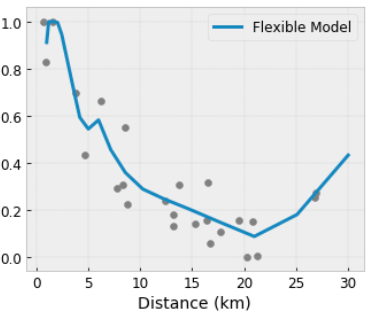
\includegraphics[height=3.5cm]{img/mon1} }}%
	\hspace{0.7cm}
	\subfloat[]{{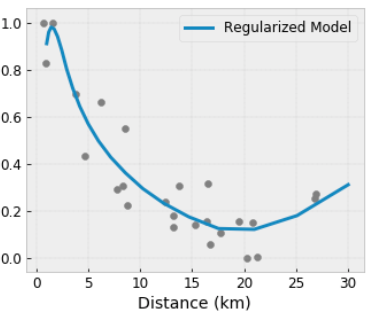
\includegraphics[height=3.5cm]{img/mon2} }}%
	\hspace{0.7cm}
	\subfloat[]{{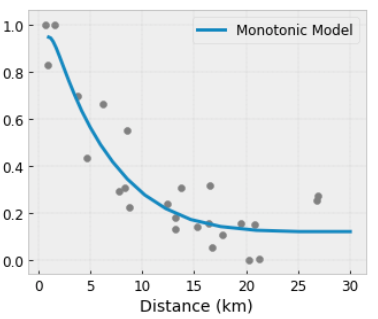
\includegraphics[height=3.5cm]{img/mon3} }}%
	\caption{The monotonic model (c) ensures that the output only decreases with respect to an input; models (a) and (b) fail in this regard (\url{https://www.tensorflow.org/lattice/overview}).}%
	\label{Fig:mon1}%
\end{figure}

To implement the constraints in the regression objective, Gupta et al. then relax strict monotonicity to monotonicity `by allowing equality in the adjacent parameter constraints' (p. 13). The updated monotonic lattice regression objective then looks the following:
\begin{align}
arg\ \underset{\theta}{min} \sum_{i = 1}^{n} \ell(y_i, \theta^T \phi(x_i)) + R(\theta)\ \mathrm{s.t.}\ A\theta \leq b.
\label{Eq:monlatreg}
\end{align}

The pairwise constraints for the lattice output $\theta$ is written as $A\theta \leq b$, whereby $A$ is a sparse matrix with one row per constraint and one $1$ and $-1$ per row. $A$ enables the specification of each individual covariate, wheter it should be constrained or unconstrained. To further constrain the fitted function in linear ways (for instance by $f(x) \geq 0$) additional linear constraints can be imposed through $A\theta \leq b$.

\subsubsection{Calibration}\label{Sec:cal}

As a way to increase accuracy, \citep{gupta2016monotonic} propose a method for transforming each covariate before they are supplied to the lattice function $f(x)$. This poses an alternative to refining the lattice by increasing the hyperparameter $M_d$, as this would be inefficient on a larger scale. \textit{Feature calibration} is an automated one-dimensional pre-processing operation $c_d[x_d]$, calibrating each of the \textit{d} covariates of $x \in D$. For continous data the authors present a one-dimensional monotonic piecewise linear function. For categorical data they propose a function for mapping each category to a real value in $[0, M_d - 1]$. Furthermore there is a suggestion of two methods to handle missing values by using a calibration approach. Now, to learn a calibrated monotonic lattice, calibration functions $c_d(\cdot)$ and lattice parameters $\theta$ are simultaneously optimized. This requires the following adjustment of the regression objective:
\begin{equation}
arg\ \underset{\theta, \alpha}{min} \sum_{i = 1}^{n} \ell(y_i, \theta^T \phi(c(x_i, \alpha))) + R(\theta)\ 
\mathrm{s.t.}\ A\theta \leq b\ \mathrm{and}\ \tilde{A}\alpha \leq b.
\label{Eq:calregobj}
\end{equation}
The vector function $c(x;\alpha)$ maps a feature vector $x$ to the lattice function $\theta^T\phi(x)$ and entails the \textit{d}th component function $c_d(x[d];\alpha^{(d)})$, which is a calibration function depending on the parameter $\alpha^{(d)}$ and the \textit{d}th component of $x$. As before $A$ denotes the monotonicity constraint, while $\tilde{A}$ does the same for each pair of adjacent calibration parameters of the calibration functions  $c(x;\alpha)$. We leave our review of lattice calibration at that. For a far more detailed description see \cite{gupta2016monotonic}; furthermore an neural network implementation (\textit{deep lattice networks}) of the theory briefly sketched in this section can be found in \citep{you2017deep}. 
\newpage
\section{Experiment Set-up}\label{Sec:Exp}

In this section we give an overview on the data used for the experiment, its processing and how it was split. More importantly, we outline the specifications of the modeling process and the evaluation method for performance assessment. 

\subsection{Data Sets and Preprocessing}

To conduct our experiment we use four credit scoring data sets. There are on the one hand two data sets obtained from \textit{Kaggle}: the 2010 \textit{PAKDD data mining challenge} data set\footnote{ \url{https://www.kaggle.com/c/pakdd2010-dataset/}}  (PAK) and the \textit{Give Me Some Credit competition} data set\footnote{ \url{http://www.kaggle.com/c/GiveMeSomeCredit}} (GMC). On the other hand we make use of two well-known UCI Machine Learning Library data sets, the \textit{Default of Credit Card Clients} data set (TCD) from Taiwanese bank customers \citep{yeh2009comparisons} and the \textit{South German credit} data set (GER), which is a reviewed version of the very common \textit{German credit} data set \citep{groemping2019south}. A brief overview on the data is given in Tab. \ref{tab:ov}. Each data set contains customer data from financial institutions. All sets are composed of a mixture of socio-economic information from the customer (i.e. age, education, maritial status), information from their loan inquiry (i.e. amount, duration) and an assessment of whether the customer failed to repay his loan. 

\begin{table}[!htb]
	\begin{center}
		\small
		\begin{tabularx}{0.95\textwidth}{@{} l *{5}{d{2.0}} @{}}
			\toprule
			Data Set & \mc{Prior default}  & \mc{Observations} & \mc{Number of} & \mc{Number of} &  \mc{Missing} \\
			&           \MC{risk}     &                       & \MC{variables}   & \MC{selected vars.} & \MC{Values} \\
			\midrule
			GER & 0.30 & 1,000 & 21 & 16 & No \\
			GMC & 0.07 & 150,000 & 12 & 11 & Yes  \\
			PAK & 0.26 & 50,000 & 54 & 11 & Yes  \\
			TCD & 0.22 & 30,000 & 25 & 17 & No  \\
			\addlinespace
			\bottomrule
		\end{tabularx}
	\end{center}
	\caption{Overview data sets}
	\label{tab:ov}
\end{table}

The first step for data processing is to make a decision about variable selection, as our lattice models requires a low amount ($n \leq 20$) of covariates.\footnote{ In addition, the computational resources for performing the experiment were rather restriced.} The main criteria for this selection are ($i$.) correlation, see the exemplary correlation plot in Appendix Fig. \ref{Fig:corrplot}, ($ii$.) and comparability, which aims to have similar variables for all data sets. Tab. \ref{tab:ov} shows the reduction of variables for each data set. As a next step we apply standard preprocessing operations as imputation of missing values by mean/mode replacement. In addition we transform the data type of every variable to be numeric, since the lattice model requires tensor shaped input data. We do not normalize the data, as none of the models requires such an operation. For the partitioning of the data we apply a simple $80/20$ train/test split, no validation or cross validation, to keep computing effort low.

\begin{figure}[htb!]
		\centering
		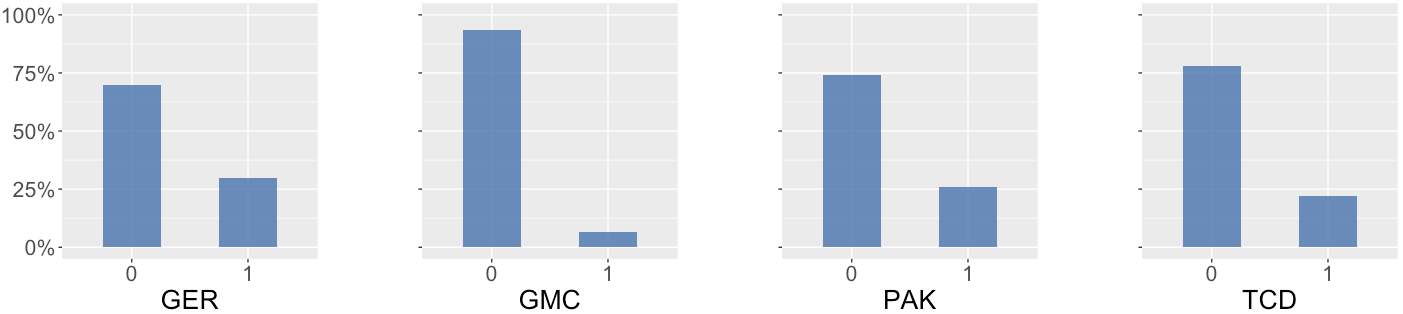
\includegraphics[width=1\textwidth]{img/defhist} % first figure itself
		\caption{The distribution of credit default for each data set.}
		\label{Fig:defhist}
\end{figure}

\subsection{Modeling and Evaluation}

The goal of this thesis is to explore lattice based models. To asses its performance, we set up an experiment in which we compare a nonlinear generalized additive model
(GAM), also referred to as lattice model, and a random forrest classifier. The algorithms are applied in a credit scoring domain on a classification problem: each of the above introduced data sets contains a binary class label for each client that determines if there is a prior risk of some kind of default or not (see Fig. \ref{Fig:defhist}). We renamed the target variable for each data set to `default' and since we are facing a binary outcome we set the value for `customer likely defaults' to $y = 1$ and for `customer likely not defaults' to $y = 0$. We chose a random forrest classifier for the comparison, as it is commonly used for credit scoring \citep{baesens2003benchmarking}, \citep{lessmann2015benchmarking}. Due to computational restrictions we forwent tuning the hyperparameters of the models. To deploy the lattice model we set up an interface to call the Tensor Flow Lattice Python library, as the experiment was run in an \textsf{R} environment. A full description of each model can be found in the accompanying \textsf{R}-script. The following gives a brief overview on the most important parameters and aspects of each model:

\subsubsection*{Calibrated Lattice Model}

Among a set of hyperparameters our, `nonlinear generalized additive model (GAM), also called a calibrated linear model in the TensorFlow Lattice' \citep[Sec.~8]{wang2020deontological}, requires a detailed specification for calibration. As we saw in Sec. \ref{Sec:cal}, a lattice model first applies piecewise-linear and categorical calibration on each input variable. The calibration function $c_d(x[d]; \alpha^{(d)})$ is parametrized by $K$ ($\alpha^{(d)} \in [0, M_d - 1]^K$, with $K$ differing for continous and categorical variables), which in simple terms determines the spacing of $c_d(\cdot)$ (\cite{gupta2016monotonic} give a detailed explanation of the calibrator on pp. 26). The amount of keypoints $K$ set and the type of spacing (by quantiles, linearly or manually) has to be specified for every variable of each data set. Our decision making about the parametrization of $c(\cdot)$ was guided by the distribution of the individual variables; if e.g. a variable had a strong skew and outliers, we would pick a higher value for $K$ and a quantile spacing. The specification for every variable and data set can be looked at in the feature configs \textsf{Python} file. 

\begin{figure}[htb!]
	\centering
	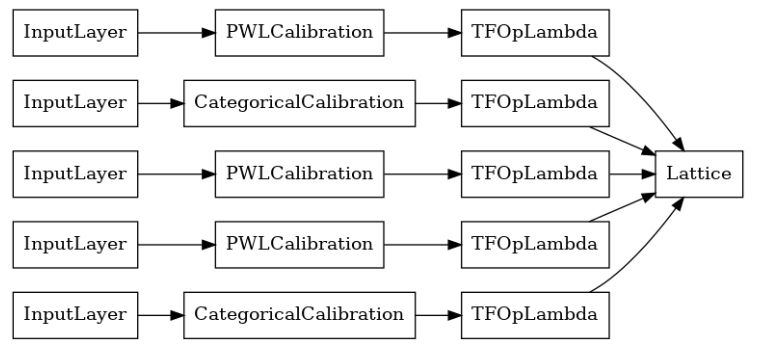
\includegraphics[width=0.65\textwidth]{img/lat}
	\caption{A simplified version of our model}
	\label{Fig:lat}
\end{figure}

There are two further important per-variable configurations entailed in this file: lattice size and monotonicity. The first we kept mostly at a default value of $2$ for the vast majority of variables, mainly to keep computational effort low. For monotonicity we again looked at variable distribution behaviour, to decide if it makes sense to apply monotonicity and whether it should be in- or decreasing. Simple charts of the variables as in Appendix Fig. \ref{Fig:ovplot} were helpful for decisions.

After calibration a lattice layer non-linearly fuses the calibrated variables, see Fig. \ref{Fig:lat}. As a regulizer for the calibration we chose the Hessian, and for making the lattice more linear we used the Torsion regulizer, both set to a value of $0.01$. Further parameters included\textit{ binary crossentropy} loss function and \textit{Adam} optimizer; a \textit{learning rate} of $0.01$, a rather large \textit{batch size} of $128$ and a rather small \textit{epoch size} of $25$, both for computational reasons.

\subsubsection*{Random Forrest}

Our random forest model of choice contains three potential tuning parameters:  a value for the number of trees, a value for the number of data points that are required for a node to split and a value for the number of predictors that will be randomly sampled at each split. We set the tree parameter at $1000$, the minimum node size parameter to $3$ and the last one at $null$. A more detailed explanation of the model can be found in \citep{breiman2001random}.

\subsubsection*{Evaluation}

Both of the introduced models were then applied to all of the credit scoring data sets. For the assessment of each classifier we chose \textit{AUC} as evaluation metric, since it is a well established metric for this kind of classification problem \citep{lessmann2015benchmarking}.

For the comparison of the performance of two classifiers on multiple datasets it is recommended to perform a statistical test on the obtained evaluation metrics, rather then just averaging over them \citep{japkowicz2011evaluating}. For our comparison of the AUC values of both models we therefore conducted \textit{Wilcoxon's Signed-Rank test}, following the approach of \citep[Sec.~6.6]{japkowicz2011evaluating}. For this test the $H_0$-hypothesis is that both classifiers perform equally as good; we are thus going to try to show, that one classifier performs better than the other one. 
\medskip

Wilcoxon's Signed-Rank test works the following way: for each pair of AUC values the difference $d_i$ is taken. These get ranked, respectively their absolute values; if a tie occurs, an average rank will be assigned to the tied values. Then a sum of ranks is calculated:
\begin{align*}
W_{s1} = \sum_{i=1}^{n} I(d_i > 0) \mathrm{rank}(d_i) + \frac{1}{2} \sum_{i=1}^{n} I(d_i = 0)\mathrm{rank}(d_i),  \\	
W_{s2} = \sum_{i=1}^{n} I(d_i < 0) \mathrm{rank}(d_i) + \frac{1}{2} \sum_{i=1}^{n} I(d_i = 0)\mathrm{rank}(d_i). 
\end{align*}

With these sums a test statistic can be calculated as $T_{wilcox}  = \mathrm{min}(W_{s1}, W_{s2}).$ To verify the rejection of $H_0$, critical values for $n < 25$ can be looked up from a table, otherwise the $T_{wilcox}$ distribution can be approximated. For a more detailed description of the test procedure see \citep[p.~234]{japkowicz2011evaluating}.

\newpage
\section{Results}\label{Sec:Results}

As summary of the results of our experiment is provided in Tab. \ref{tab:res}. On a first glance there is no larger difference in the performance of both classifier, with random forrest doing slightly better in most of cases. But the averaging over the $\mathrm{AUC}_{ts}$ values is deceiving. Applying Wilcoxon's Signed-Rank test on the result leaves us with a \textit{p}-value of $0.25$; we therefore cannot reject the $H_0$-hypothesis. Based on the given data and employing the above sketched models we cannot state that one classifier performs better then the other. This result aligns with those of \citep[Sec.~10]{gupta2016monotonic} and \citep[Sec.~8]{wang2020deontological}, who both test calibrated lattice models against a random forrest classifier. The former tune their hyperparameters, our experiment set up is more comparable to the one of Wang \& Gupta. As we saw in Sec. \ref{Sec:covshift}, they also used the TCD data set. Our experiment can therefore partially be seen as a confirmation of their experiment, since we only reproduced it with a different classifier for comparison. \medskip

\begin{table}[!htb]
	\begin{center}
		\small
		\begin{tabular}[t]{lrrrrr}
		\toprule
		\multicolumn{1}{c}{ } & \multicolumn{2}{c}{\textbf{Lattice}} & \multicolumn{2}{c}{\textbf{Tree}} & \multicolumn{1}{c}{Diff} \\
		\cmidrule(l{3pt}r{3pt}){2-3} \cmidrule(l{3pt}r{3pt}){4-5} \cmidrule(l{3pt}r{3pt}){6-6}
				 & $\mathrm{AUC}_{tr} $ & $\mathrm{AUC}_{ts}$  & $\mathrm{AUC}_{tr}$ & $\mathrm{AUC}_{ts}$ & $\mathrm{AUC}_{ts}$\\
		\midrule
		GER & 0.7523 & \textbf{0.7737} & 1.0000 & 0.7643 & 0.0094\\
		GMC & 0.8367 & 0.8438 & 0.9998 & \textbf{0.8585} & -0.0146\\
		PAK & 0.5481 & 0.5422 & 0.9371 & \textbf{0.5733} & -0.0311\\
		TCD & 0.7316 & 0.7271 & 0.9997 &\textbf{ 0.7728} & -0.0458\\
		\midrule
		Average & 0.7171 & 0.7216 & 0.9841 & 0.7422 & \\ 
		\addlinespace
		\bottomrule
		\end{tabular}
	\caption{Resulting $AUC$ values from the experiment}
	\label{tab:res}
	\end{center}
\end{table}
\vspace*{-0.6cm}
For improving the experiment set-up to hopefully obtain even more sound results, a couple of measures could be taken:
\begin{itemize}
	\setlength\itemsep{-0.05em}
	\item[-] The statistical test could be altered, so that we actually reject the $H_0$-Hypothesis. An alternative would be an Equivalence test \citep{walker2011understanding}.
	\item[-] The number of credit scoring data sets could be increased.
	\item[-] The data could be split in a more sophisticated manner, for instance by cross-validation.
	\item[-] Other types of classifiers could be introduced for comparison
	\item[-] The grid could be tuned for all of the hyperparameters.
\end{itemize}


\section{Conclusions}\label{Sec:Conc}

In this paper we gave a brief introduction into the lattice regression framework and its extensions. We furthermore gave an example of how covariate shift can affect credit scoring applications and proposed to use a lattice model as a mitigation strategy. In our case study we then showed that a monotonic calibrated lattice model does not perform worse on credit data then a default random forrest model. 

The proposed ameliorations in Sec. \ref{Sec:Results} can be seen as a first step to improve the study. As a next step it would be interesting to compare the model with one or more covariate shift correction algorithms presented in Sec. \ref{Sec:Relwork}.  In addition, another feature of the lattice model should be explored further: the proclaimed enhanced interpretability of the model through the lattice structure \citep{gupta2016monotonic}. Recently, interpretability is becoming a topic of concern, as so called `black box'-models are criticized for being unsuitable to be used in ethically crucial situations due to lack of transparency \citep{rudin2019stop}. 

Throughout the paper it should have shown that covariate shift touches deeply on the problem of inductive reasoning. When \citep{shimodaira2000improving} introduced the concept of covariate shift, he claimed that is it exclusively caused by model misspecification and that it would disappear for a correct model. But when do we ever know the correct specification of a model? `In reality, however, good fitting models with a modest number of parameters are hard to obtain except for very simple applications.' \citep[p.~202]{quionero2009dataset} says Shimodaira. The question `How do we justify generalization for our model from train data to test data?' will continously loom in the background.




% ----------------
% --- appendix ---
% ----------------
\appendix

% literature
\newpage
\addcontentsline{toc}{section}{References}
\bibliography{appendix/lit_ba20}

% figures (not mandatory)
\newpage
\section{Figures}

\begin{figure}[!htb]
	\begin{center}
		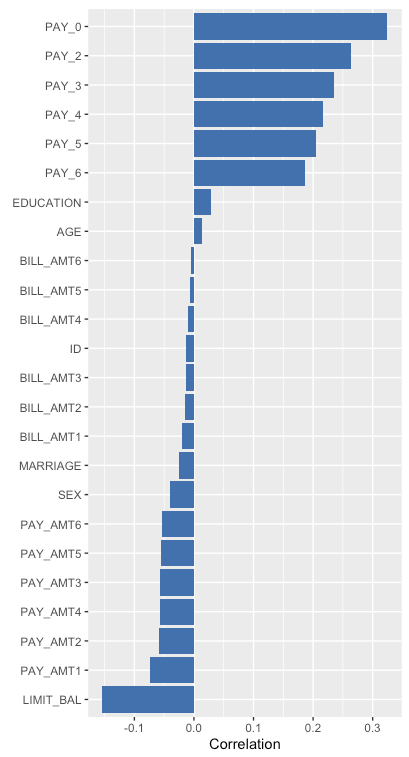
\includegraphics[width=0.5\textwidth]{img/corrplot}
		\caption{The Figure shows the correlation of the dependant with the independant covariates for TCD. We removed all `BILL' variables, `ID' and `MARRIAGE', but kept `AGE' for comparability.}
		\label{Fig:corrplot}
	\end{center}
\end{figure}

\pagebreak

\begin{figure}[!htb]
    \begin{center}
        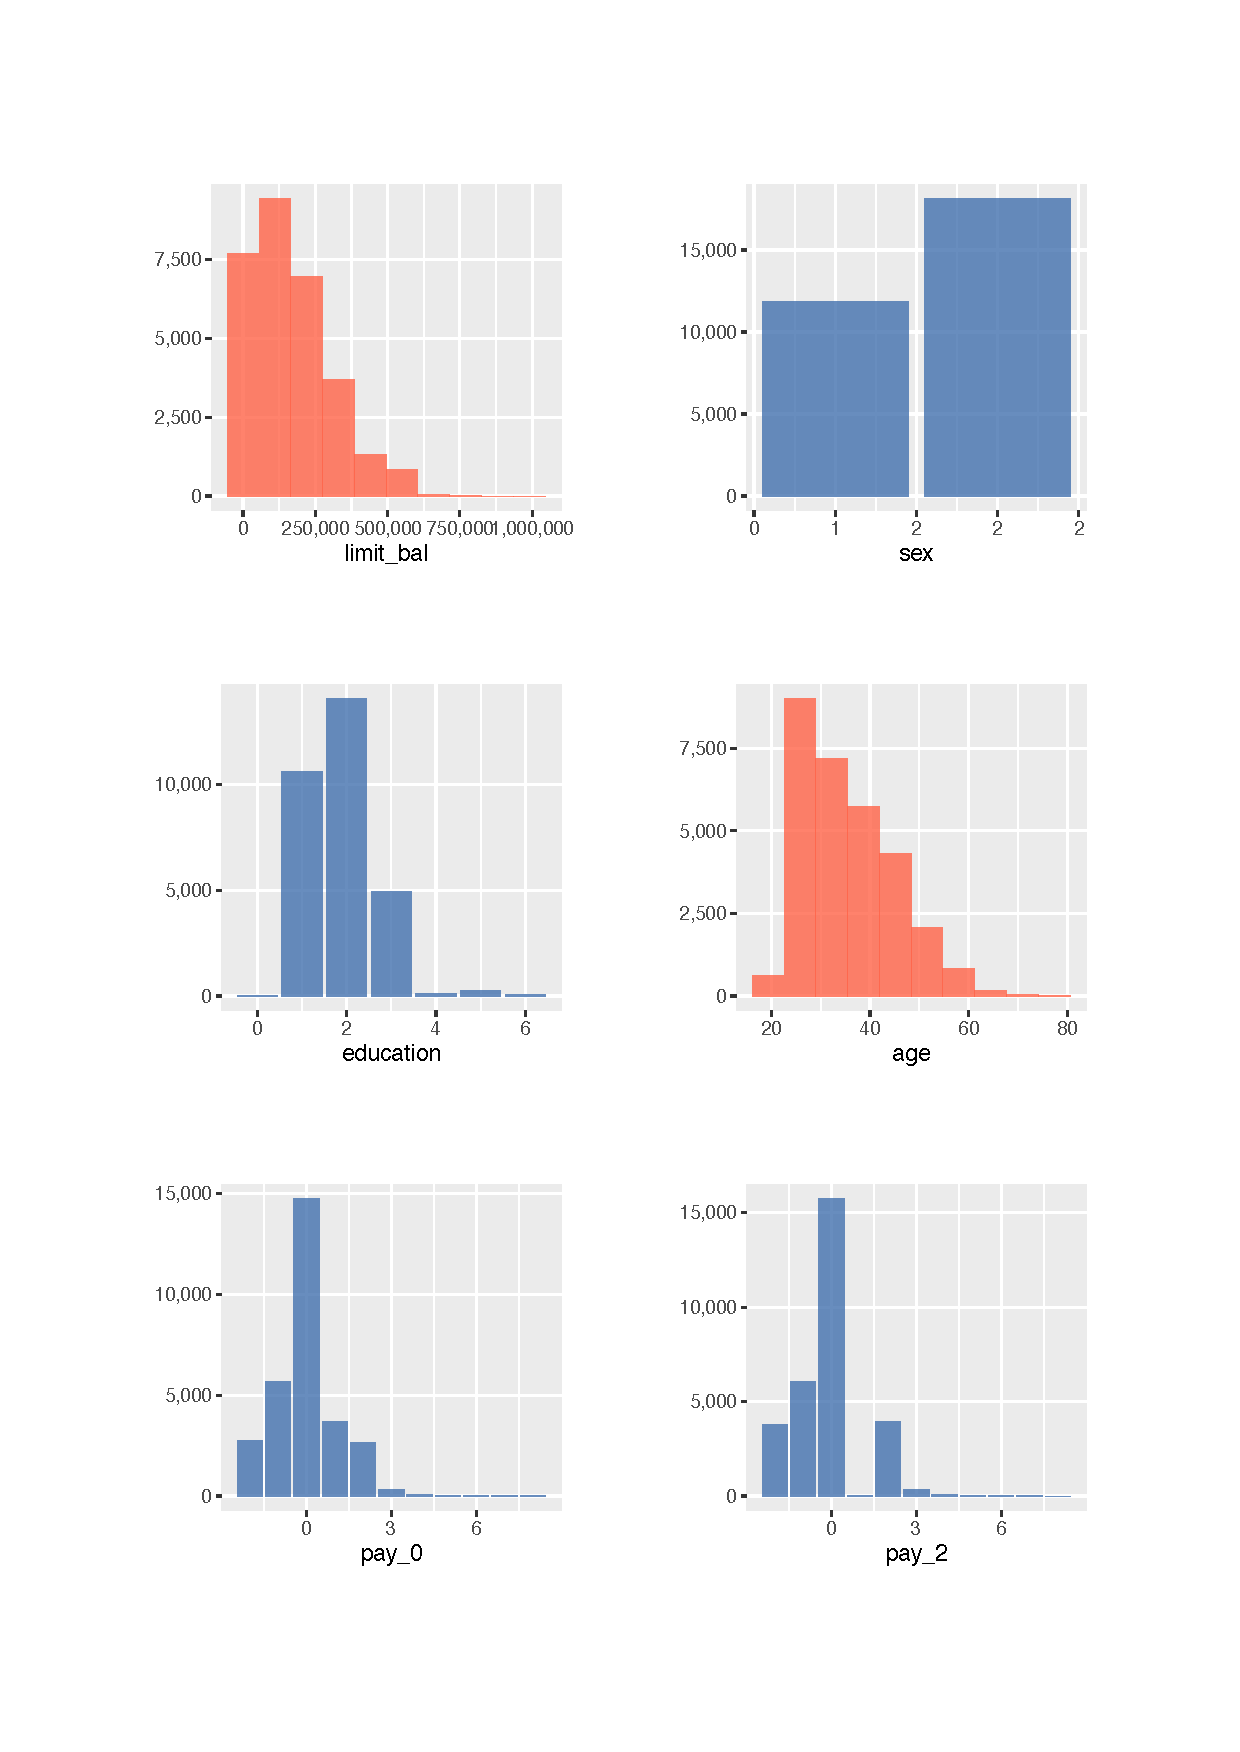
\includegraphics[width=0.9\textwidth]{img/ov_plot}
        \caption{Example plots for TCD data set}
        \label{Fig:ovplot}
    \end{center}
\end{figure}

\pagebreak

\begin{figure}[!htb]
	\begin{center}
		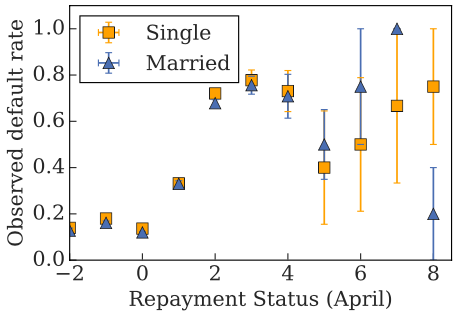
\includegraphics[width=0.65\textwidth]{img/gup3}
		\caption{Training examples for credit data \citep{wang2020deontological}}
		\label{Fig:gup3}
	\end{center}
\end{figure}

 
% --------------------------------------------
% --- last page: Declaration of Authorship ---
% --------------------------------------------

%\newpage
%\thispagestyle{empty}
%%{\Large{\bf Declaration of Authorship}}\vspace{0.5cm}

\section*{Declaration of Authorship}

I, Jonathan Schmitz, hereby declare that I have not previously submitted the present work for other examinations. I wrote this work independently. All sources, including sources from the Internet, that I have reproduced in either an unaltered or modified form (particularly sources for texts, graphs, tables and images), have been acknowledged by me as such. I understand that violations of these principles will result in proceedings regarding deception or attempted deception.
\vspace{1cm}

Berlin, May 17$th$, 2021 \vspace{0.3cm}

\underline{\hspace{5cm}} \medskip

Jonathan Schmitz



\label{key}\end{document}
